% answers.tex —— 1989 年·全国卷·文科 · 参考答案与详细解析片段
% 由 tools/generate_projects.py 依来源总账自 1989/1989_数学真题_全国文_试题.md + 1989/1989_数学真题_全国文_解析正文.md + 1989/1989_数学真题_全国文_答案要点.md 生成，勿手改（改源 MD 后重跑）


\begin{gktip}
本稿为根据已核题面推导的解析草稿。固定源未附答案或解析，不能将本稿视为来源原文或官方解答；独立盲核尚未完成。
\end{gktip}

\begin{answer}
\gksolhead{1}{}

\textbf{题目}：

如果 $I=\{a,b,c,d,e\}$，$M=\{a,c,d\}$，$N=\{b,d,e\}$，其中 $I$ 是全集，那么 $\overline M\cap\overline N$ 等于\mbox{（　　）}

（A）$\varnothing$　　（B）$\{d\}$　　（C）$\{a,c\}$　　（D）$\{b,e\}$

\Needspace{4\baselineskip}
\textbf{解析}

相对于全集 $I$，有 $\overline M=\{b,e\}$，$\overline N=\{a,c\}$，两者无公共元素，交集为空集。选 A。注意题面是两个补集的交集，不能丢失横线后改算 $M\cap N$。

\gkanswer{答案：A}

\end{answer}
\begin{answer}
\gksolhead{2}{}

\textbf{题目}：

与函数 $y=x$ 有相同图象的一个函数是\mbox{（　　）}

（A）$y=\sqrt{x^2}$　　（B）$y=\dfrac{x^2}{x}$

（C）$y=a^{\log_a x}$，其中 $a>0$，$a\ne1$

（D）$y=\log_a a^x$，其中 $a>0$，$a\ne1$

\Needspace{4\baselineskip}
\textbf{解析}

A 为 $y=|x|$；B 在 $x=0$ 处没有定义；C 的定义域为 $x>0$。D 中 $a^x>0$ 对全部实数 $x$ 成立，且 $\log_a(a^x)=x$，定义域和值均与 $y=x$ 一致，选 D。

\gkanswer{答案：D}

\end{answer}
\begin{answer}
\gksolhead{3}{}

\textbf{题目}：

如果圆锥的底面半径为 $\sqrt2$，高为 $2$，那么它的侧面积是\mbox{（　　）}

（A）$4\sqrt3\pi$　　（B）$2\sqrt2\pi$　　（C）$2\sqrt3\pi$　　（D）$4\sqrt2\pi$

\Needspace{4\baselineskip}
\textbf{解析}

圆锥的母线长 $l=\sqrt{(\sqrt2)^2+2^2}=\sqrt6$，侧面积 $\pi rl=\pi\sqrt2\sqrt6=2\sqrt3\pi$，选 C。结果量纲为长度的平方。

\gkanswer{答案：C}

\end{answer}
\begin{answer}
\gksolhead{4}{}

\textbf{题目}：

已知 $\{a_n\}$ 是等比数列，如果 $a_1+a_2=12$，$a_2+a_3=-6$，且 $S_n=a_1+a_2+\cdots+a_n$，那么 $\displaystyle\lim_{n\to\infty}S_n$ 的值等于\mbox{（　　）}

（A）$8$　　（B）$16$　　（C）$32$　　（D）$48$

\Needspace{4\baselineskip}
\textbf{解析}

由 $a_2+a_3=q(a_1+a_2)$ 得 $q=-1/2$，进而 $a_1(1+q)=12$，所以 $a_1=24$。因 $|q|<1$，部分和的极限为 $a_1/(1-q)=16$，选 B。

\gkanswer{答案：B}

\end{answer}
\begin{answer}
\gksolhead{5}{}

\textbf{题目}：

如果 $(1-2x)^7=a_0+a_1x+a_2x^2+\cdots+a_7x^7$，那么 $a_1+a_2+\cdots+a_7$ 的值等于\mbox{（　　）}

（A）$-2$　　（B）$-1$　　（C）$0$　　（D）$2$

\Needspace{4\baselineskip}
\textbf{解析}

令 $x=0$ 得 $a_0=1$，令 $x=1$ 得全部系数之和为 $-1$。所求为 $-1-a_0=-2$，选 A。

\gkanswer{答案：A}

\end{answer}
\begin{answer}
\gksolhead{6}{}

\textbf{题目}：

如果 $|\cos\theta|=\dfrac15$，$\dfrac52\pi<\theta<3\pi$，那么 $\sin\dfrac\theta2$ 的值等于\mbox{（　　）}

（A）$-\dfrac{\sqrt{10}}5$　　（B）$\dfrac{\sqrt{10}}5$　　（C）$-\dfrac{\sqrt{15}}5$　　（D）$\dfrac{\sqrt{15}}5$

\Needspace{4\baselineskip}
\textbf{解析}

\Needspace{5\baselineskip}
在 $5\pi/2<\theta<3\pi$ 上，$\cos\theta<0$，故 $\cos\theta=-1/5$。同时 $5\pi/4<\theta/2<3\pi/2$，半角的正弦为负。因此

\nopagebreak[4]
\[
\sin\frac\theta2=-\sqrt{\frac{1-\cos\theta}{2}}=-\frac{\sqrt{15}}5\text{。}
\]

选 C。

\gkanswer{答案：C}

\end{answer}
\begin{answer}
\gksolhead{7}{}

\textbf{题目}：

直线 $2x+3y-6=0$ 关于点 $(1,-1)$ 对称的直线是\mbox{（　　）}

（A）$3x-2y+2=0$　　（B）$2x+3y+7=0$

（C）$3x-2y-12=0$　　（D）$2x+3y+8=0$

\Needspace{4\baselineskip}
\textbf{解析}

中心对称变换将 $(x,y)$ 映到 $(2-x,-2-y)$，代入原直线得 $2(2-x)+3(-2-y)-6=0$，整理为 $2x+3y+8=0$，选 D。

\gkanswer{答案：D}

\end{answer}
\begin{answer}
\gksolhead{8}{}

\textbf{题目}：

已知球的两个平行截面的面积分别为 $5\pi$ 和 $8\pi$，它们位于球心的同一侧，且相距为 $1$，那么这个球的半径是\mbox{（　　）}

（A）$4$　　（B）$3$　　（C）$2$　　（D）$5$

\Needspace{4\baselineskip}
\textbf{解析}

设球半径为 $R$，面积较小的截面到球心的距离为 $d_1$，另一个为 $d_2$。同侧且相距 1 给出 $d_1-d_2=1$；由 $R^2-d_1^2=5$、$R^2-d_2^2=8$ 得 $(d_1-d_2)(d_1+d_2)=3$。于是 $d_1=2$、$d_2=1$，$R^2=9$，故 $R=3$，选 B。

\gkanswer{答案：B}

\end{answer}
\begin{answer}
\gksolhead{9}{}

\textbf{题目}：

由数字 $1,2,3,4,5$ 组成没有重复数字的五位数，其中偶数共有\mbox{（　　）}

（A）$60$ 个　　（B）$48$ 个　　（C）$36$ 个　　（D）$24$ 个

\Needspace{4\baselineskip}
\textbf{解析}

个位只能为 2 或 4，两种选法；其余四个不同数字任意排列，有 $4!$ 种。共有 $2\cdot4!=48$ 个，选 B。

\gkanswer{答案：B}

\end{answer}
\begin{answer}
\gksolhead{10}{}

\textbf{题目}：

如果双曲线 $\dfrac{x^2}{64}-\dfrac{y^2}{36}=1$ 上一点 $P$ 到它的右焦点的距离是 $8$，那么点 $P$ 到它的右准线的距离是\mbox{（　　）}

（A）$10$　　（B）$\dfrac{32\sqrt7}{7}$　　（C）$2\sqrt7$　　（D）$\dfrac{32}{5}$

\Needspace{4\baselineskip}
\textbf{解析}

双曲线的 $a=8$、$b=6$，故 $c=10$、离心率 $e=c/a=5/4$。到相应焦点和准线的距离满足 $PF=e\,d$，所以 $d=8/(5/4)=32/5$，选 D。

\gkanswer{答案：D}

\end{answer}
\begin{answer}
\gksolhead{11}{}

\textbf{题目}：

如果 $|x|\le\dfrac\pi4$，那么函数 $f(x)=\cos^2x+\sin x$ 的最小值是\mbox{（　　）}

（A）$\dfrac{\sqrt2-1}{2}$　　（B）$-\dfrac{1+\sqrt2}{2}$　　（C）$-1$　　（D）$\dfrac{1-\sqrt2}{2}$

\Needspace{4\baselineskip}
\textbf{解析}

令 $t=\sin x$，则 $-\sqrt2/2\le t\le\sqrt2/2$，$f(x)=1-t^2+t$。这是开口向下的抛物线，闭区间上的最小值在端点取得。比较两端得最小值 $1/2-\sqrt2/2=(1-\sqrt2)/2$，选 D。

\gkanswer{答案：D}

\end{answer}
\begin{answer}
\gksolhead{12}{}

\textbf{题目}：

已知 $f(x)=8+2x-x^2$，如果 $g(x)=f(2-x^2)$，那么 $g(x)$\mbox{（　　）}

（A）在区间 $(-1,0)$ 上是减函数　　（B）在区间 $(0,1)$ 上是减函数

（C）在区间 $(-2,0)$ 上是增函数　　（D）在区间 $(0,2)$ 上是增函数

\Needspace{4\baselineskip}
\textbf{解析}

代入复合函数得到 $g(x)=8+2x^2-x^4$，$g'(x)=4x(1-x^2)$。在 $(-1,0)$ 上导数为负，在 $(0,1)$ 上为正；在 $(-2,0)$、$(0,2)$ 内导数均变号。因此只有 A 成立。

\gkanswer{答案：A}

\end{answer}
\begin{answer}
\gksolhead{13}{}

\textbf{题目}：

给定三点 $A(1,0)$，$B(-1,0)$，$C(1,2)$，那么通过点 $A$ 并且与直线 $BC$ 垂直的直线方程是 $\underline{\hspace{6em}}$。

\Needspace{4\baselineskip}
\textbf{解析}

直线 BC 的斜率为 $(2-0)/(1+1)=1$，所求垂线斜率为 $-1$。过 $(1,0)$ 的方程为 $y=-(x-1)$，即 $x+y-1=0$。

\gkanswer{答案：$x+y-1=0$}

\end{answer}
\begin{answer}
\gksolhead{14}{}

\textbf{题目}：

不等式 $|x^2-3x|>4$ 的解集是 $\underline{\hspace{7em}}$。

\Needspace{4\baselineskip}
\textbf{解析}

绝对值不等式分为 $x^2-3x>4$ 或 $x^2-3x<-4$。前者等价于 $(x-4)(x+1)>0$，给出 $x<-1$ 或 $x>4$；后者左移后为 $x^2-3x+4<0$，其判别式为 $-7$ 且二次项系数为正，无实解。解集为 $(-\infty,-1)\cup(4,+\infty)$。

\gkanswer{答案：$(-\infty,-1)\cup(4,+\infty)$}

\end{answer}
\begin{answer}
\gksolhead{15}{}

\textbf{题目}：

函数 $y=\dfrac{e^x-1}{e^x+1}$ 的反函数的定义域是 $\underline{\hspace{6em}}$。

\Needspace{4\baselineskip}
\textbf{解析}

原函数在全部实数上连续且严格递增，导数为 $2e^x/(e^x+1)^2>0$；当 $x\to-\infty$、$x\to+\infty$ 时分别趋于 $-1$、$1$，端点均不取。因此原函数值域、也即反函数定义域为 $(-1,1)$。

\gkanswer{答案：$(-1,1)$}

\end{answer}
\begin{answer}
\gksolhead{16}{}

\textbf{题目}：

已知 $A$ 和 $B$ 是两个命题，如果 $A$ 是 $B$ 的充分条件，那么 $B$ 是 $A$ 的 $\underline{\hspace{4em}}$ 条件；$\overline A$ 是 $\overline B$ 的 $\underline{\hspace{4em}}$ 条件。

\Needspace{4\baselineskip}
\textbf{解析}

“A 是 B 的充分条件”表示 $A\Rightarrow B$，所以 B 是 A 的必要条件。其逆否命题为 $\overline B\Rightarrow\overline A$，所以 $\overline A$ 是 $\overline B$ 的必要条件。两空均填“必要”，不额外假定逆命题成立。

\gkanswer{答案：必要；必要}

\end{answer}
\begin{answer}
\gksolhead{17}{}

\textbf{题目}：

已知 $0<a<1$，$0<b<1$，$a^{\log_b(x-3)}<1$，那么 $x$ 的取值范围是 $\underline{\hspace{6em}}$。

\Needspace{4\baselineskip}
\textbf{解析}

因 $0<a<1$，有 $a^t<1$ 当且仅当 $t>0$。因此 $\log_b(x-3)>0$；又 $0<b<1$，这等价于 $0<x-3<1$。故 $3<x<4$，已包含对数的真数约束。

\gkanswer{答案：$3<x<4$}

\end{answer}
\begin{answer}
\gksolhead{18}{}

\textbf{题目}：

如图，$P$ 是二面角 $\alpha$-$AB$-$\beta$ 棱 $AB$ 上的一点，分别在 $\alpha$、$\beta$ 上引射线 $PM$、$PN$，如果 $\angle BPM=\angle BPN=45^\circ$，$\angle MPN=60^\circ$，那么二面角 $\alpha$-$AB$-$\beta$ 的大小是 $\underline{\hspace{4em}}$。
\nopagebreak[4]
\begin{center}% 依据固定源印刷页35；投影图不表示角度或比例。
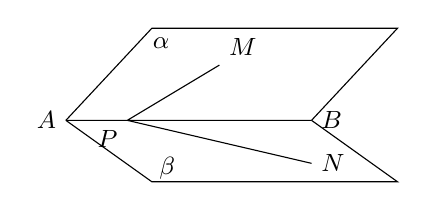
\begin{tikzpicture}[scale=0.78,font=\small]
  \coordinate (A) at (0,0);
  \coordinate (B) at (4,0);
  \coordinate (P) at (1,0);
  \coordinate (M) at (2.5,0.9);
  \coordinate (N) at (4,-0.7);
  \draw (A)--(1.4,1.5)--(5.4,1.5)--(B);
  \draw (A)--(1.4,-1)--(5.4,-1)--(B);
  \draw (A)--(B) (P)--(M) (P)--(N);
  \node[left] at (A) {$A$};
  \node[right] at (B) {$B$};
  \node[below left] at (P) {$P$};
  \node[above right] at (M) {$M$};
  \node[right] at (N) {$N$};
  \node at (1.55,1.25) {$\alpha$};
  \node at (1.65,-0.78) {$\beta$};
\end{tikzpicture}
\end{center}
\nopagebreak[4]
\Needspace{4\baselineskip}
\textbf{解析}

\Needspace{5\baselineskip}
以 PB 的方向为单位向量 $\boldsymbol e$，令两面内分别垂直于 PB 并指向相应半平面的单位向量为 $\boldsymbol u$、$\boldsymbol v$，二面角为 $\delta\in[0,\pi]$。由两射线与 PB 均成 $45^\circ$，它们的单位方向分别是 $(\boldsymbol e+\boldsymbol u)/\sqrt2$、$(\boldsymbol e+\boldsymbol v)/\sqrt2$。于是

\nopagebreak[4]
\[
\cos60^\circ=\frac{1+\boldsymbol u\cdot\boldsymbol v}{2}
=\frac{1+\cos\delta}{2}\text{。}
\]

所以 $\cos\delta=0$，二面角为 $90^\circ$。不能直接把投影图上的角当作实际二面角量取。

\gkanswer{答案：$90^\circ$}

\end{answer}
\begin{answer}
\gksolhead{19}{}

\textbf{题目}：

设复数 $z=(1-\sqrt3 i)^5$，求 $z$ 的模和辐角的主值。

\Needspace{4\baselineskip}
\textbf{解析}

$1-\sqrt3 i$ 的模为 2，辐角可取 $-\pi/3$。由棣莫弗公式，$z$ 的模为 $2^5=32$，辐角可取 $-5\pi/3$，在 $[0,2\pi)$ 内的主值为 $\pi/3$。

\gkanswer{答案：$|z|=32$，$\arg z=\dfrac\pi3$}

\end{answer}
\begin{answer}
\gksolhead{20}{}

\textbf{题目}：

\Needspace{5\baselineskip}
证明：

\nopagebreak[4]
\[
\tan\frac{3x}{2}-\tan\frac{x}{2}=\frac{2\sin x}{\cos x+\cos2x}\text{。}
\]

\Needspace{0.65\textheight}

\Needspace{4\baselineskip}
\textbf{解析}

\Needspace{5\baselineskip}
在各式有定义的 $x$ 上，用正切差公式及积化和差得

\nopagebreak[4]
\[
\tan\frac{3x}{2}-\tan\frac{x}{2}
=\frac{\sin x}{\cos\frac{3x}{2}\cos\frac{x}{2}}
=\frac{2\sin x}{\cos2x+\cos x}\text{。}
\]

其中 $2\cos(3x/2)\cos(x/2)=\cos2x+\cos x$，故两边分母非零的约束相同，无需补入原式无定义的点。

\gkanswer{答案：见解析版}

\end{answer}
\begin{answer}
\gksolhead{21}{}

\textbf{题目}：

如图，在平行六面体 $ABCD-A_1B_1C_1D_1$ 中，已知 $AB=5$，$AD=4$，$AA_1=3$，$AB\perp AD$，$\angle A_1AB=\angle A_1AD=\dfrac\pi3$。

（1） 求证：顶点 $A_1$ 在底面 $ABCD$ 的射影 $O$ 在 $\angle BAD$ 的平分线上；

（2） 求这个平行六面体的体积。
\nopagebreak[4]
\begin{center}% 依据固定源印刷页35；斜棱平行六面体及射影，不按未给定视角量角。
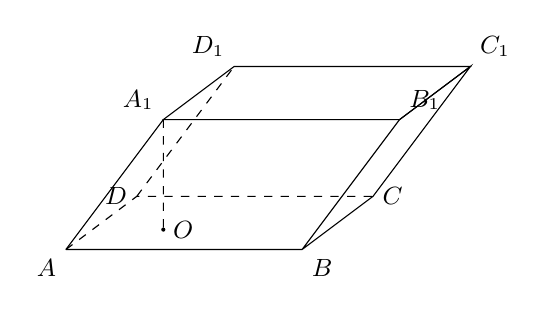
\begin{tikzpicture}[scale=0.75,font=\small]
  \coordinate (A) at (0,0);
  \coordinate (B) at (4,0);
  \coordinate (D) at (1.2,0.9);
  \coordinate (C) at (5.2,0.9);
  \coordinate (A1) at (1.65,2.2);
  \coordinate (B1) at (5.65,2.2);
  \coordinate (D1) at (2.85,3.1);
  \coordinate (C1) at (6.85,3.1);
  \coordinate (O) at (1.65,0.3375);
  \draw (A)--(B)--(C)--(C1)--(B1)--(B) (A)--(A1);
  \draw (A1)--(B1)--(C1)--(D1)--cycle;
  \draw[dashed] (A)--(D)--(C) (D)--(D1) (A1)--(O);
  \fill (O) circle (1pt) node[right] {$O$};
  \node[below left] at (A) {$A$};
  \node[below right] at (B) {$B$};
  \node[right] at (C) {$C$};
  \node[left] at (D) {$D$};
  \node[above left] at (A1) {$A_1$};
  \node[above right] at (B1) {$B_1$};
  \node[above right] at (C1) {$C_1$};
  \node[above left] at (D1) {$D_1$};
\end{tikzpicture}
\end{center}
\nopagebreak[4]
\Needspace{4\baselineskip}
\textbf{解析}

\gksubpart{（1）}

以 A 为原点，AB、AD 的方向为相互垂直的 x、y 轴，底面法线为 z 轴。由 $AA_1=3$ 及两个 $60^\circ$ 夹角，$A_1$ 的 x、y 坐标均为 $3\cos60^\circ=3/2$。射影 $O=(3/2,3/2,0)$，因此在底面角 BAD 的内角平分线 $x=y\ge0$ 上。

\gksubpart{（2）}

由空间距离公式，高为 $h=\sqrt{3^2-(3/2)^2-(3/2)^2}=3\sqrt2/2$。

底面是边长 5、4 的矩形，所以平行六面体体积为 $V=5\cdot4\cdot h=30\sqrt2$，量纲为给定长度单位的三次方。

\gkanswer{答案（1）：$O$ 在 $\angle BAD$ 的内角平分线上}

\gkanswer{答案（2）：$30\sqrt2$}

\end{answer}
\begin{answer}
\gksolhead{22}{}

\textbf{题目}：

\Needspace{5\baselineskip}
用数学归纳法证明：

\nopagebreak[4]
\[
(1\cdot2^2-2\cdot3^2)+(3\cdot4^2-4\cdot5^2)+\cdots
+\bigl[(2n-1)(2n)^2-2n(2n+1)^2\bigr]
=-n(n+1)(4n+3)\text{。}
\]

\Needspace{4\baselineskip}
\textbf{解析}

令等式左边为 $S_n$。当 $n=1$ 时，$S_1=4-18=-14=-1\cdot2\cdot7$，等式成立。

\Needspace{5\baselineskip}
假设 $S_k=-k(k+1)(4k+3)$。第 $k+1$ 个括号可直接展开为

\nopagebreak[4]
\[
(2k+1)(2k+2)^2-(2k+2)(2k+3)^2
=-12(k+1)^2-2(k+1)\text{。}
\]

\Needspace{5\baselineskip}
所以

\nopagebreak[4]
\[
S_{k+1}=-k(k+1)(4k+3)-12(k+1)^2-2(k+1)
=-(k+1)(k+2)(4k+7)\text{。}
\]

这正是 $n=k+1$ 时的式子，故由数学归纳法对所有正整数 n 成立。

\gkanswer{答案：见解析版}

\end{answer}
\begin{answer}
\gksolhead{23}{}

\textbf{题目}：

已知 $a>0$，$a\ne1$，试求使方程 $\log_a(x-ak)=\log_{a^2}(x^2-a^2)$ 有解的 $k$ 的取值范围。

\Needspace{4\baselineskip}
\textbf{解析}

\Needspace{5\baselineskip}
对数定义域要求 $x-ak>0$ 且 $x^2-a^2>0$。因 $\log_{a^2}t=\tfrac12\log_at$，无论 a 在 1 的哪一侧，原等式均等价于

\nopagebreak[4]
\[
x-ak=\sqrt{x^2-a^2}>0\text{。}
\]

\Needspace{5\baselineskip}
平方后得到 $2akx=a^2(k^2+1)$。$k=0$ 时矛盾；$k\ne0$ 时唯一候选为

\nopagebreak[4]
\[
x=\frac{a(k^2+1)}{2k},\qquad x-ak=\frac{a(1-k^2)}{2k}\text{。}
\]

由后者严格为正，得 $k<-1$ 或 $0<k<1$。上述两区间内 $x^2-a^2=\dfrac{a^2(k^2-1)^2}{4k^2}>0$，且 $x-ak>0$，故候选满足未平方的等式，条件也充分。$k=\pm1$ 令真数为零，应排除。范围为 $(-\infty,-1)\cup(0,1)$。

\gkanswer{答案：$k\in(-\infty,-1)\cup(0,1)$}

\end{answer}
\begin{answer}
\gksolhead{24}{}

\textbf{题目}：

给定椭圆方程 $\dfrac{x^2}{b^2}+\dfrac{y^2}{a^2}=1$（$a>b>0$），求与这个椭圆有公共焦点的双曲线，使得以它们的交点为顶点的四边形面积最大，并求相应的四边形的顶点坐标。

\Needspace{4\baselineskip}
\textbf{解析}

\Needspace{5\baselineskip}
记 $c^2=a^2-b^2$，原椭圆的焦点为 $(0,\pm c)$。非退化共焦双曲线只能写为

\nopagebreak[4]
\[
\frac{y^2}{A^2}-\frac{x^2}{B^2}=1,\qquad A^2+B^2=c^2,\quad A>0,\ B>0\text{。}
\]

\Needspace{5\baselineskip}
令 $t=A^2/c^2\in(0,1)$。联立两曲线，可得交点的坐标平方为 $x^2=b^2(1-t)$、$y^2=a^2t$。四个交点的正负号独立，组成矩形，面积为

\nopagebreak[4]
\[
S=4ab\sqrt{t(1-t)}\le2ab\text{。}
\]

等号当且仅当 $t=1/2$，此时 $A^2=B^2=c^2/2$，所求双曲线为 $y^2-x^2=(a^2-b^2)/2$，四个顶点为 $(\pm b/\sqrt2,\pm a/\sqrt2)$，最大面积为 $2ab$。条件 $a>b>0$ 保证上述双曲线非退化。

\gkanswer{答案：$y^2-x^2=\dfrac{a^2-b^2}{2}$；顶点为 $(\pm\dfrac b{\sqrt2},\pm\dfrac a{\sqrt2})$（正负号独立组合），最大面积为 $2ab$}

\end{answer}